%%%%%%%%%%%%%%%%%%%%%%%%%%%%%%%%%%%%%
%                                   %
% Compile with XeLaTeX and biber    %
%                                   %
% Questions or comments:            %
%                                   %
% joshua dot mcneill at uga dot edu %
%                                   %
%%%%%%%%%%%%%%%%%%%%%%%%%%%%%%%%%%%%%

\documentclass{beamer}
  % Read in standard preamble (cosmetic stuff)
  %%%%%%%%%%%%%%%%%%%%%%%%%%%%%%%%%%%%%%%%%%%%%%%%%%%%%%%%%%%%%%%%
% This is a standard preamble used in for all slide documents. %
% It basically contains cosmetic settings.                     %
%                                                              %
% Joshua McNeill                                               %
% joshua dot mcneill at uga dot edu                            %
%%%%%%%%%%%%%%%%%%%%%%%%%%%%%%%%%%%%%%%%%%%%%%%%%%%%%%%%%%%%%%%%

% Beamer settings
% \usetheme{Berkeley}
\usetheme{CambridgeUS}
% \usecolortheme{dove}
% \usecolortheme{rose}
\usecolortheme{seagull}
\usefonttheme{professionalfonts}
\usefonttheme{serif}
\setbeamertemplate{bibliography item}{}

% Packages and settings
\usepackage{fontspec}
  \setmainfont{Charis SIL}
\usepackage{hyperref}
  \hypersetup{colorlinks=true,
              allcolors=blue}
\usepackage{graphicx}
  \graphicspath{{../../figures/}}
\usepackage[normalem]{ulem}
\usepackage{enumerate}

% Document information
\author{M. McNeill}
\title[FREN2001]{Français 2001}
\institute{\url{joshua.mcneill@uga.edu}}
\date{}

%% Custom commands
% Lexical items
\newcommand{\lexi}[1]{\textit{#1}}
% Gloss
\newcommand{\gloss}[1]{`#1'}
\newcommand{\tinygloss}[1]{{\tiny`#1'}}
% Orthographic representations
\newcommand{\orth}[1]{$\langle$#1$\rangle$}
% Utterances (pragmatics)
\newcommand{\uttr}[1]{`#1'}
% Sentences (pragmatics)
\newcommand{\sent}[1]{\textit{#1}}
% Base dir for definitions
\newcommand{\defs}{../definitions}


  % Packages and settings

  % Document information
  \subtitle[Activités]{Nos activités}

\begin{document}
  % Read in the standard intro slides (title page and table of contents)
  \begin{frame}
    \titlepage
    \tiny{Office: % Basically a variable for office hours location
Gilbert 121\\
          Office hours: % Basically a variable for office hours
 lundi, mercredi, vendredi 10:10--11:10
}
  \end{frame}

  \begin{frame}{Annonces}
    \begin{itemize}
      \item L'atelier d'écoute, le 12 septembre
      \item[] \gloss{Listening workshop, September 12th}
      \item Rendez le devoir 1, le 12 septembre
      \item[] \gloss{Turn in homework, September 12th}
    \end{itemize}
  \end{frame}

  \begin{frame}{}
    \begin{center}
      \Large Quiz
    \end{center}
  \end{frame}

  \begin{frame}{Revue des verbes -er}
    Par exemple:
    \begin{center}
      \begin{tabular}{l | l l | l l}
  \multicolumn{5}{c}{regarder \gloss{to look at, to watch}} \\
      & \multicolumn{2}{l |}{singulier} & \multicolumn{2}{l}{pluriel} \\
  \hline
  1re & je         & regarde            & nous        & regardons \\
  2e  & tu         & regardes           & vous        & regardez \\
  \hline
  3e  & il (masc)  &                    & ils (masc)  & \\
      & elle (fem) & regarde            & elles (fem) & regardent \\
      & on         &                    &             & \\
\end{tabular}

    \end{center}
  \end{frame}

  \begin{frame}{Les associations des verbes -er}
    \centering
    écouter

    \uncover<2->{
      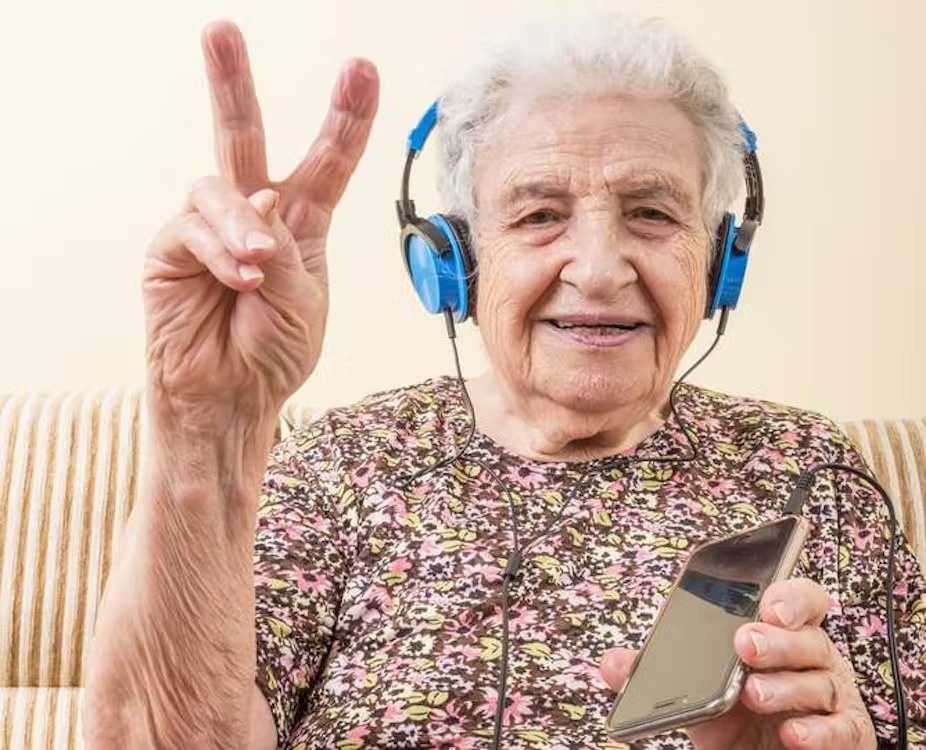
\includegraphics[scale=0.2]{ecouter.jpg}
    }
  \end{frame}

  \begin{frame}{Les associations des verbes -er}
    \centering
    jouer

    \uncover<2->{
      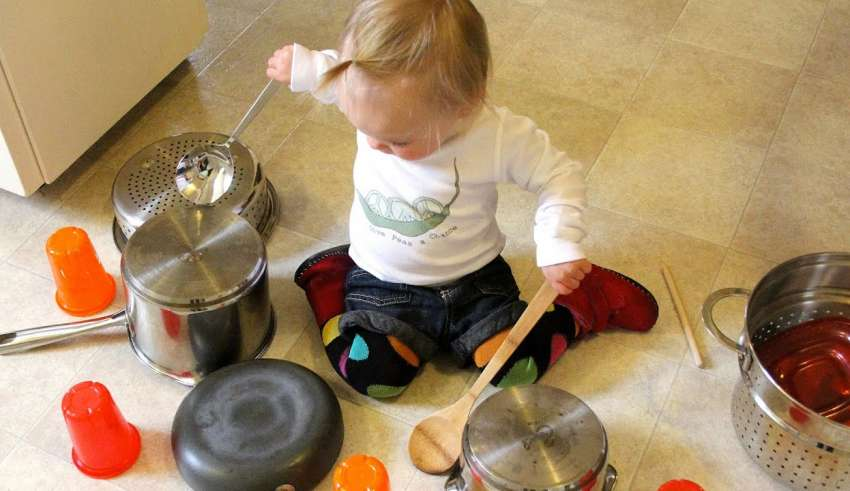
\includegraphics[scale=0.4]{jouer.jpg}
    }
  \end{frame}

  \begin{frame}{Les associations des verbes -er}
    \centering
    préparer

    \uncover<2->{
      \includegraphics[scale=1]{préparer.jpg}
    }
  \end{frame}

  \begin{frame}{Les associations des verbes -er}
    \centering
    parler

    \uncover<2->{
      
\includegraphics[scale=0.25]{parler.jpg}
    }
  \end{frame}

  \begin{frame}{Les associations des verbes -er}
    \centering
    travailler

    \uncover<2->{
      
\includegraphics[scale=0.75]{travailler.jpg}
    }
  \end{frame}

  \begin{frame}{Les associations des verbes -er}
    \begin{columns}
      \column{0.5\textwidth}
        \begin{center}
          inviter
        \end{center}
      \column{0.5\textwidth}
        \begin{center}
          \uncover<2->{
            
\includegraphics[scale=0.37]{inviter.jpg}
          }
        \end{center}
    \end{columns}
  \end{frame}

  \begin{frame}{Les habitudes}
    \gloss{With a partner, take turns explaining \alert{when} the following people do the following things.
    For example: \emph{toi / regarder la télé, Je regarde la télé le dimanche}}
    \begin{enumerate}
      \item toi / retrouver des amis
      \item toi et tes amis / jouer au foot
      \item ton père / préparer le dîner
      \item toi / écouter la radio
      \item ton frère ou ta sœur / téléphoner aux parents
      \item tes parents / travailler
    \end{enumerate}
  \end{frame}

  \begin{frame}{Cette semaine}
    \gloss{With a partner, take turns saying what you'll be doing this week.
    For example:}
    \begin{description}
      \item[E1:] Vendredi soir, je regarde un film avec mes amis.
      \item[E2:] Moi, vendredi soir, je téléphone à mes parents.
    \end{description}

  \end{frame}

  \begin{frame}{}
    \begin{center}
      \Large Questions?
    \end{center}
  \end{frame}
\end{document}
